\documentclass[margin=5mm, tikz]{standalone}
\usepackage[utf8x]{inputenc}
\usepackage{tikz}
\begin{document}
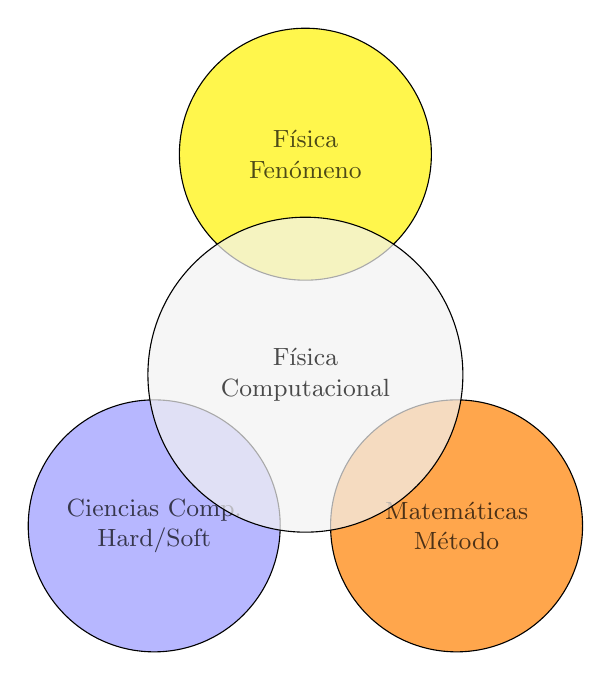
\begin{tikzpicture}[scale=0.8, font = \small]
\begin{scope}[fill opacity=0.7]


\draw [fill=yellow, thin] (0,3.5) circle (2);
\draw [align=center] (0,3.5) node {Física \\ Fenómeno};
\draw [fill=blue!40, thin] (-2.4,-2.4) circle (2);
\draw [align = center] (-2.4,-2.4) node {Ciencias Comp. \\ Hard/Soft};

\draw [fill=orange, thin] (2.4,-2.4) circle (2);
\draw [align=center] (2.4,-2.4) node {Matemáticas \\ Método};

\draw [fill=gray!10, thin] (0,0) circle (2.5);
\draw [align = center] (0,0) node {Física \\ Computacional};

\end{scope}
\end{tikzpicture}
\end{document}